% Copyright 2004 by Till Tantau <tantau@users.sourceforge.net>.
%
% In principle, this file can be redistributed and/or modified under
% the terms of the GNU Public License, version 2.
%
% However, this file is supposed to be a template to be modified
% for your own needs. For this reason, if you use this file as a
% template and not specifically distribute it as part of a another
% package/program, I grant the extra permission to freely copy and
% modify this file as you see fit and even to delete this copyright
% notice. 
\documentclass{beamer}
\usepackage{bbm}
\usepackage{lipsum}
\usepackage{enumitem}
\usepackage{pifont}
\usepackage{tikz}
\usepackage{lmodern}
\usepackage{commath}
\usepackage{bbm} %package for using the bbm fonts in math environment
\usetikzlibrary{calc}
\usepackage{xparse} 
\usetikzlibrary{calc}
\logo{\color{red}\rule{.5cm}{.5cm}}
\newcommand{\btVFill}{\vskip0pt plus 1filll}
\usepackage{afterpage}
\usepackage{xcolor}

%\usepackage{xcolor}
%\usepackage{tikz}
%\usetikzlibrary{shadows}
\newlength{\tmpShadow}
\newcommand{\MyShadow}[2]{%
	\settowidth{\tmpShadow}{#1}
	\addtolength{\tmpShadow}{.1em}
	\raisebox{-0.25ex}{\textcolor{gray!70}{#1}}%
	\kern-\tmpShadow%
	\textcolor{#2}{#1}%
}


\tikzset{
	invisible/.style={opacity=0,text opacity=0},
	visible on/.style={alt=#1{}{invisible}},
	alt/.code args={<#1>#2#3}{%
		\alt<#1>{\pgfkeysalso{#2}}{\pgfkeysalso{#3}} 
	},
}
\tikzset{
	background fill/.style={fill=#1},
	background fill/.default={white},
	fill on/.style={alt=#1{}{background fill}},
}
\tikzset{
	background draw/.style={draw=#1},
	background draw/.default={white},
	draw on/.style={alt=#1{}{background draw}},
}
\tikzset{
	background filldraw/.style args={#1 filled by #2}{draw=#1, fill=#2},
	background filldraw/.default=white filled by white,
	filldraw on/.style={alt=#1{}{background filldraw}},
}
\tikzset{highlighting/.style={
		append after command={
			\pgfextra{
				\path[rounded corners,
				background draw=red,
				draw on=<#1>,
				overlay] ($(\tikzlastnode.south west)+(-0.015,-0.1)$) % to have some offset
				rectangle ($(\tikzlastnode.north east)+(0.015,0.07)$);
			}   
		}
	}
}
\NewDocumentCommand{\highlight}{r<> m}{%
	\tikz[baseline=(A.base)] 
	\node[highlighting=#1,
	inner sep=0pt] (A) {#2};%
}

%\newcommand*{\MyShadowBullet}{\tikz \draw [baseline, fill=blue,draw=blue,circular drop shadow] circle (2pt);}
%\newcommand*{\MyBallBullet}{\tikz \draw [baseline, ball color=red, draw=red] circle (2pt);}

\newcommand{\nologo}{\setbeamertemplate{logo}{}} % command to set the logo to nothing
\usepackage{multicol}
\newcommand\tab[1][1cm]{\hspace*{#1}}

%gets rid of bottom navigation bars
%\setbeamertemplate{footline}[frame number]{}
%gets rid of bottom navigation symbols
\setbeamertemplate{navigation symbols}{}
%gets rid of footer
%will override 'frame number' instruction above
%comment out to revert to previous/default definitions
%\setbeamertemplate{footline}{}

\newcounter{mycounter}  
\newenvironment{noindlist}
{\begin{list}{}{\usecounter{mycounter} \labelsep=0em \labelwidth=0em \leftmargin=0em \itemindent=0em}}
	{\end{list}}

% There are many different themes available for Beamer. A comprehensive
% list with examples is given here:
% http://deic.uab.es/~iblanes/beamer_gallery/index_by_theme.html
% You can uncomment the themes below if you would like to use a different
% one:
%\usetheme{AnnArbor}
%\usetheme{Antibes}
%\usetheme{Bergen}
%\usetheme{Berkeley}
%\usetheme{Berlin}
%\usetheme{Boadilla}
%\usetheme{boxes}
%\usetheme{CambridgeUS}
%\usetheme{Copenhagen}
%\usetheme{Darmstadt}
%\usetheme{default}
%\usetheme{Frankfurt}
%\usetheme{Goettingen}
%\usetheme{Hannover}
%\usetheme{Ilmenau}
%\usetheme{JuanLesPins}
%\usetheme{Luebeck}
\usetheme{Madrid}
%\usetheme{Malmoe}
%\usetheme{Marburg}
%\usetheme{Montpellier}
%\usetheme{PaloAlto}
%\usetheme{Pittsburgh}
%\usetheme{Rochester}
%\usetheme{Singapore}
%\usetheme{Szeged}
%\usetheme{Warsaw}

%\setbeamercolor{normal text}{fg=white,bg=black!90}
%\setbeamercolor{structure}{fg=blue!80}
%\setbeamercolor{alerted text}{fg=red!85!black}
%\setbeamercolor{item projected}{use=item,fg=black,bg=item.fg!35}
%\setbeamercolor*{palette primary}{use=structure,fg=structure.fg}
%\setbeamercolor*{palette secondary}{use=structure,fg=structure.fg!95!black}
%\setbeamercolor*{palette tertiary}{use=structure,fg=structure.fg!90!black}
%\setbeamercolor*{palette quaternary}{use=structure,fg=structure.fg!95!black,bg=black!80}
%\setbeamercolor*{framesubtitle}{fg=white}
%\setbeamercolor*{block title}{parent=structure,bg=black!60}
%\setbeamercolor*{block body}{fg=black,bg=blue!10}
%\setbeamercolor*{block title alerted}{parent=alerted text,bg=black!15}
%\setbeamercolor*{block title example}{parent=example text,bg=black!15}


\title{Feature assessment and selection using sparse clustering}

% A subtitle is optional and this may be deleted
%\subtitle{Optional Subtitle}

\author{Avgoustinos~Vouros\inst{1}}
% - Give the names in the same order as the appear in the paper.
% - Use the \inst{?} command only if the authors have different
%   affiliation.

\institute[] % (optional, but mostly needed)
{
  \inst{1}%
  PhD student, \\Department of Computer Science,\\
  University of Sheffield\\
  \vspace{5mm}
  \noindent Supervised by Prof Eleni Vasilaki
  %\and
  %\inst{2}%
  %Department of Theoretical Philosophy\\
  %University of Elsewhere
}

\date{} %removes the date
% - Use the \inst command only if there are several affiliations.
% - Keep it simple, no one is interested in your street address.

%\date{Conference Name, 2013}
% - Either use conference name or its abbreviation.
% - Not really informative to the audience, more for people (including
%   yourself) who are reading the slides online

%\subject{Theoretical Computer Science}
% This is only inserted into the PDF information catalog. Can be left
% out. 

% If you have a file called "university-logo-filename.xxx", where xxx
% is a graphic format that can be processed by latex or pdflatex,
% resp., then you can add a logo as follows:

\pgfdeclareimage[height=1cm]{university-logo}{university-logo}
\logo{\pgfuseimage{university-logo}}

% Delete this, if you do not want the table of contents to pop up at
% the beginning of each subsection:
\AtBeginSubsection[]
{
  \begin{frame}<beamer>{Outline}
    \tableofcontents[]
  \end{frame}
}

% Let's get started
\begin{document}

\begin{frame}
  \titlepage
\end{frame}

%\begin{frame}{Acknowledgements}
%	Original slides created by: 
%	\begin{itemize}
%		\item Eleni Vasilaki (Prof)
%		\item Tiago V. Gehring (PhD)
%	\end{itemize}
%	\vspace{5mm}
%	Revised and modified slides created by:
%	\begin{itemize}
%		\item Avgoustinos Vouros
%	\end{itemize}	
%\end{frame}

%%%%%%%%%%%%%%%%%%%%%%%%%%%%%%%%%%%%%%%%%%%%%%%%%%%%%%%%%

\begin{frame}{Contents}
	\begin{itemize}[label={\MyShadow{$\bullet$}{black!80}}]
		\item The K-Means Algorithm (Lloyd's)
		\vspace{3mm}
		\item Sparse K-Means
		\vspace{3mm}
		\begin{itemize}[label={\MyShadow{$\bullet$}{black!80}}]
			\item Theory
			\begin{itemize}[label={\MyShadow{$\star$}{black!80}}]
				\item Regression (quick)
			\end{itemize}	
			\vspace{3mm}
			\item Algorithm
			\vspace{3mm}
			\item Tuning
			\begin{itemize}[label={\MyShadow{$\star$}{black!80}}]
				\item Gap Statistic
			\end{itemize}				
		\end{itemize}
		\vspace{1mm}
		\item Ongoing Research
	\end{itemize}
\end{frame}


\begin{frame}[plain,c]
%\frametitle{A first slide}
	\vspace{1mm}
	\begin{center}
		\Huge The K-Means Algorithm\\
		\Huge (Lloyd's)
	\end{center}
\end{frame}


{\nologo
\begin{frame}{The K-Means Algorithm (Lloyd's)}
	\begin{figure}[H]
		\centering
		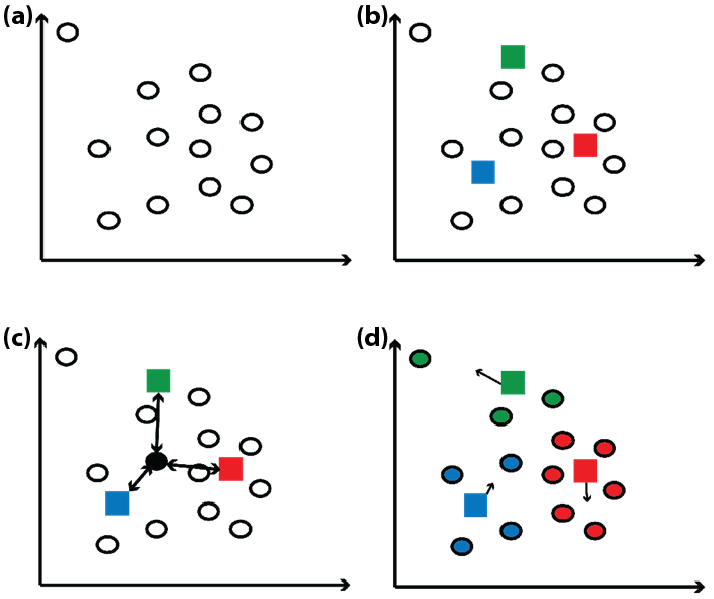
\includegraphics[width=0.7\textwidth]{figures/km2}
	\end{figure}

	\begin{tiny}
		\begin{noindlist}
			\item $[1]$ Lloyd, Stuart. ``Least squares quantization in PCM.'' IEEE transactions on information theory 28.2 (1982): 129-137.
		\end{noindlist}
	\end{tiny}
\end{frame}


\begin{frame}{The K-Means Algorithm (Lloyd's)}
	Minimize: 
	\begin{align}\nonumber
		WCSS &= \sum_{k=1}^{K}\sum_{\binom{i=1}{x_{i:} \in c_k}}^{n} \sum_{j=1}^{p}(x_{ij}-m_{kj})^2
	\end{align}	
	Maximize:
	\begin{align}\nonumber
		BCSS &= \sum_{j=1}^{p} \bigg( \sum_{i=1}^{n}(x_{ij}-M_{1j})^2 - \sum_{k=1}^{K}\sum_{\binom{i=1}{x_{i:} \in c_k}}^{n}(x_{ij}-m_{kj})^2 \bigg)	
	\end{align}			
\end{frame}


\begin{frame}{The K-Means Algorithm (Lloyd's)}
	\begin{multicols}{2}
		\textbf{Advantages:}
		\vspace{3mm}
		\begin{itemize}[label={\MyShadow{$\bullet$}{blue!80}}]
			\item Simple and easy to implement.
			\vspace{3mm}
			\item Versatile.
			\vspace{3mm}
			\item Guaranteed to converge. 
			\vspace{3mm}
			\item Invariant to data ordering.			
		\end{itemize}
		\columnbreak 
		\textbf{Disadvantages:}
		\vspace{3mm}
		\begin{itemize}[label={\MyShadow{$\bullet$}{red!80}}]
			\item Detects only spherical and well-separated clusters.
			\vspace{3mm}
			\item Sensitive to noise and outliers (Euclidean).
			\vspace{3mm}
			\item Converges to a local minimum. 			
		\end{itemize}			
	\end{multicols}
	\vspace{3mm}
	\begin{itemize}
		\centering
		\item<2-> \textbf{In general:}
	\end{itemize}
	\vspace{3mm}
	\begin{itemize}[label={\MyShadow{$\bullet$}{green!80}}]
		\centering
		\item<2-> Sensitive to initial centroids location.
		\vspace{3mm}
		\item<3->\highlight<3->{Sensitive to features (variables/attributes)}.			
	\end{itemize}	
	
	\vspace{1mm}
	\begin{tiny}
		\begin{noindlist}
			\item $[1]$ Celebi, M. Emre, Hassan A. Kingravi, and Patricio A. Vela. ``A comparative study of efficient initialization methods for the k-means clustering algorithm.'' Expert systems with applications 40.1 (2013): 200-210.
		\end{noindlist}
	\end{tiny}
\end{frame}

\begin{frame}[plain,c]
	\begin{center}
		\Huge Sparse K-Means\\
		\Huge - Theory -
	\end{center}
\end{frame}

\begin{frame}{Sparse K-Means Theory}
	\begin{align}\nonumber
		\underset{c_1,\dots,c_k,w}{maximize}& \Bigg\{ \sum_{j=1}^{p} w_{jj} \bigg( \sum_{i=1}^{n}(x_{ij}-M_{1j})^2 - \sum_{k=1}^{K}\sum_{\binom{i=1}{x_{i:} \in c_k}}^{n}(x_{ij}-m_{kj})^2 \bigg) \Bigg\}  \\ \nonumber
		\text{subject to}& \hphantom{xxxxx} \sum_{j=1}^{p} w_{jj}^{2} \leq 1 \text{,}\hphantom{x} \sum_{j=1}^{p} \abs{w_{jj}} \leq s \text{,}\hphantom{x} w_{jj} \geq 0\hphantom{x} \forall j 
	\end{align}	
	\vspace{3mm}
	\begin{itemize}[label={\MyShadow{$\bullet$}{green!80}}]
		\item<2-> w is a diagonal square $p$-by-$p$ matrix.
		\vspace{3mm}
		\item<2-> $\sum_{j=1}^{p} w_{jj}^{2} \leq 1$ is the $L_2$ penalty or ridge regression ($\norm{w}^{2} \leq 1$) $[2]$.	
		\vspace{3mm}
		\item<2-> $\sum_{j=1}^{p} \abs{w_{jj}} \leq s$ is the $L_1$ penalty or lasso regression ($\abs{w} \leq s$) $[3]$.					
	\end{itemize}	
	
	\vspace{5mm}
	\begin{tiny}
		\begin{noindlist}
			\item $[1]$ Witten, Daniela M., and Robert Tibshirani. ``A framework for feature selection in clustering.'' Journal of the American Statistical Association 105.490 (2010): 713-726.
			\item<2-> $[2]$ Hoerl, Arthur E., and Robert W. Kennard. ``Ridge regression: Biased estimation for nonorthogonal problems.'' Technometrics 12.1 (1970): 55-67.	
			\item<2-> $[3]$ Tibshirani, Robert. ``Regression shrinkage and selection via the lasso.'' Journal of the Royal Statistical Society. Series B (Methodological) (1996): 267-288.						
		\end{noindlist}
	\end{tiny}	
\end{frame}

%% REGRESSION %%%%%%%%%%%%%%%%%%%%%%%%%%%%%%%%%%%%%%%%%%%%%%%%%%%%%%%%%%%%%%%%%%%%
\begin{frame}{Regression}
	\begin{figure}[H]
		\centering
		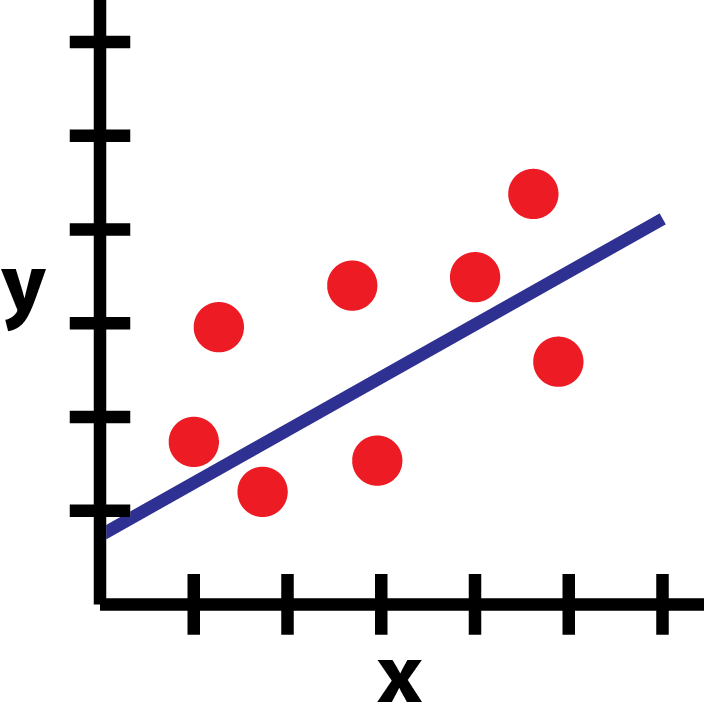
\includegraphics[width=0.3\textwidth]{figures/reg1}
	\end{figure}
	\vspace{27mm}
	\begin{tiny}
		\begin{noindlist}
			\item $[1]$ StatQuest with Josh Starmer. ``Regularization Part 1: Ridge Regression.'' YouTube. 2018. Online: \href{https://www.youtube.com/watch?v=Q81RR3yKn30}{https://www.youtube.com/watch?v=Q81RR3yKn30}.			
			\item $[2]$ StatQuest with Josh Starmer. ``Regularization Part 2: Lasso Regression.'' YouTube. 2018. Online: \href{https://www.youtube.com/watch?v=NGf0voTMlcs}{https://www.youtube.com/watch?v=NGf0voTMlcs}.						
		\end{noindlist}
	\end{tiny}		
\end{frame}

\begin{frame}{Regression}
	\begin{multicols}{2}
		\begin{itemize}
			\item<1->
				\begin{figure}[H]
					\centering
					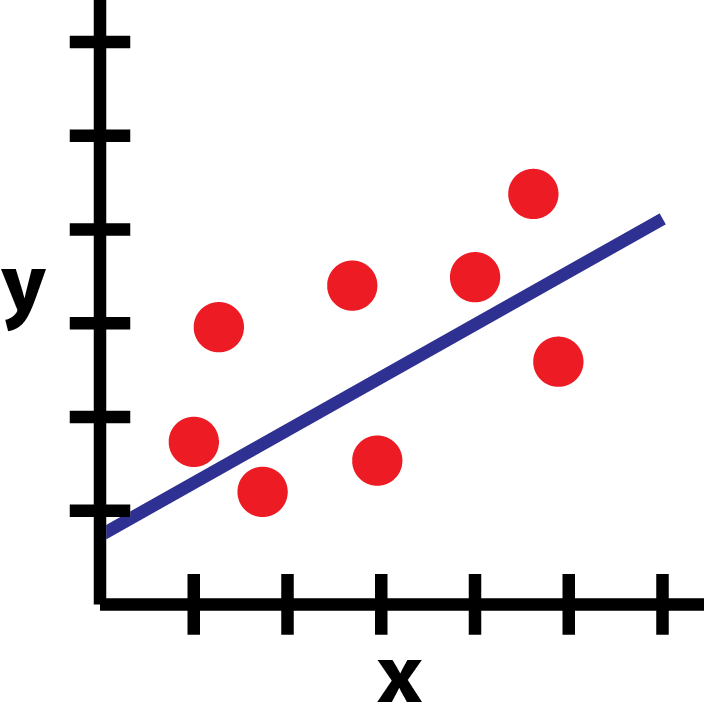
\includegraphics[width=0.3\textwidth]{figures/reg1}
				\end{figure}
			\item<1-> Line fitting using least squares:
			\item<1-> 
				\begin{align}\nonumber
					y = y_{inter} + slope * x	
				\end{align}	
			\item<1-> Least squares minimizes the sum of the squared residuals.
		\end{itemize}
	\end{multicols}	
\end{frame}

\begin{frame}{Regression}
	\begin{multicols}{2}
		\begin{itemize}
			\item<1->
			\begin{figure}[H]
				\centering
				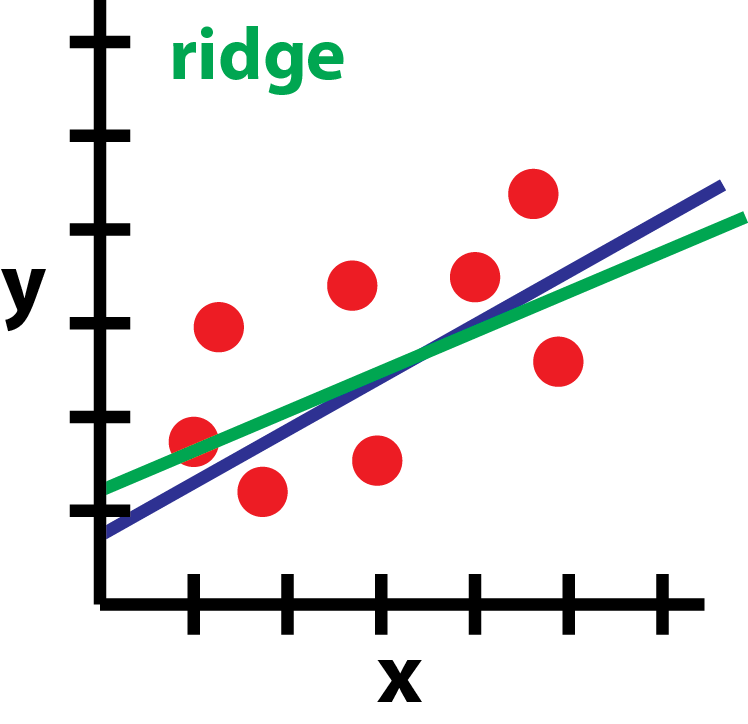
\includegraphics[width=0.3\textwidth]{figures/reg2}
			\end{figure}
			\item<1-> Line fitting using ridge regression:
			\item<1-> 
				\begin{align}\nonumber
					y = y_{inter} + slope * x \\\nonumber
					+ \lambda_2 * slope^2	
				\end{align}		
		\end{itemize}	
	\end{multicols}			
	\begin{multicols}{2}
		\begin{itemize}
			\item<2->
			\begin{figure}[H]
				\centering
				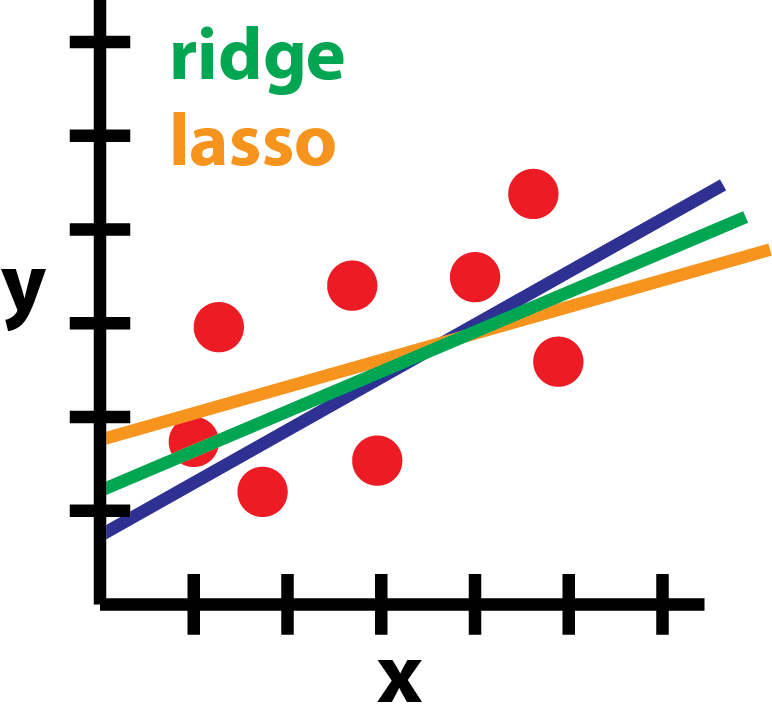
\includegraphics[width=0.3\textwidth]{figures/reg3}
			\end{figure}
			\item<2-> Line fitting using lasso regression:
			\item<2-> 
				\begin{align}\nonumber
					y = y_{inter} + slope * x \\
					+ \lambda_1 * \abs{slope}\nonumber	
				\end{align}		
		\end{itemize}	
	\end{multicols}		
\end{frame}

\begin{frame}{Regression}
	\begin{itemize}
		\item
			\begin{align}\nonumber
				 y = y_{inter} + slope * x + \lambda_2 * slope^2 \hphantom{xx} \boldmath{(a)}	
			\end{align}	
		\item
			\begin{align}\nonumber
				y = y_{inter} + slope * x + \lambda_1 * \abs{slope} \hphantom{xx} \boldmath{(b)}	
			\end{align}			
	\end{itemize}	
	\begin{figure}[H]
		\centering
		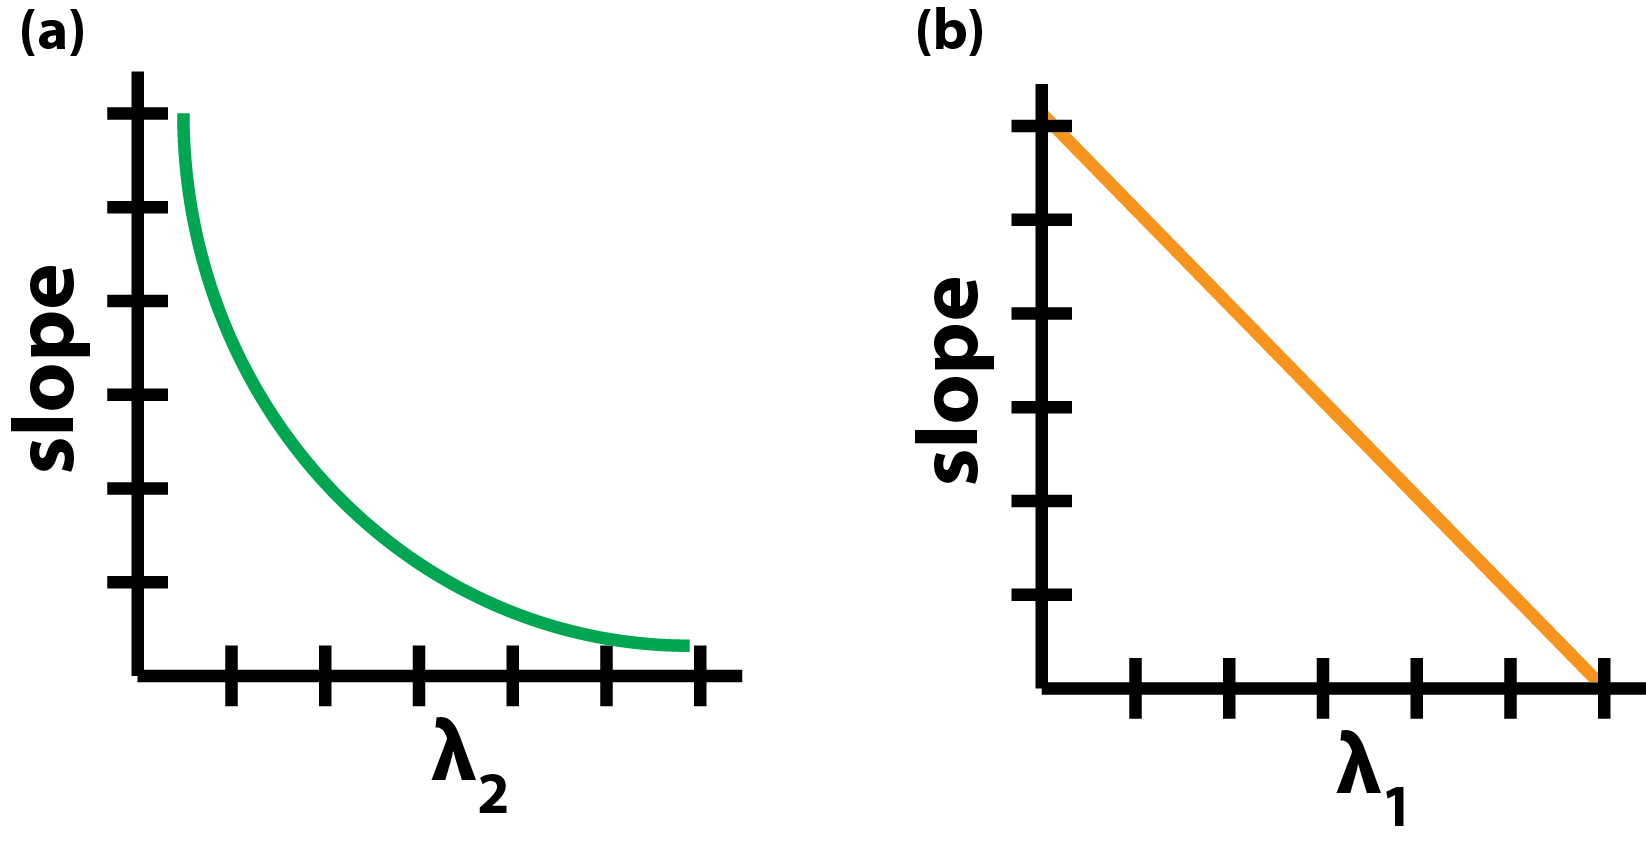
\includegraphics[width=0.8\textwidth]{figures/reg4}
	\end{figure}
\end{frame}
%% END REGRESSION %%%%%%%%%%%%%%%%%%%%%%%%%%%%%%%%%%%%%%%%%%%%%%%%%%%%%%%%%%%%%%%%%%%%

\begin{frame}{Sparse K-Means Theory}
	\begin{itemize}
		\item<1-> \begin{align}\nonumber
			\underset{c_1,\dots,c_k,w}{maximize}& \Bigg\{ \sum_{j=1}^{p} w_{jj} \bigg( \sum_{i=1}^{n}(x_{ij}-M_{1j})^2 - \sum_{k=1}^{K}\sum_{\binom{i=1}{x_{i:} \in c_k}}^{n}(x_{ij}-m_{kj})^2 \bigg) \Bigg\}  \\ \nonumber
			\text{subject to}& \hphantom{xxxxx} \sum_{j=1}^{p} w_{jj}^{2} \leq 1 \text{,}\hphantom{x} \sum_{j=1}^{p} \abs{w_{jj}} \leq s \text{,}\hphantom{x} w_{jj} \geq 0\hphantom{x} \forall j 
		\end{align}	
		\vspace{5mm}	
		\item<2-> \begin{align}\nonumber
			\underset{w}{maximize}& \Bigg\{ \sum_{j=1}^{p} w_{jj}a_j + \lambda\sum_{j=1}^{p} w_{jj}^{2} + \delta\sum_{j=1}^{p} \abs{w_{jj}} \Bigg\}
		\end{align}	
	\end{itemize}
\end{frame}

\begin{frame}{Sparse K-Means Theory}
	\begin{align}\nonumber
		\underset{w}{maximize}& \Bigg\{ \sum_{j=1}^{p} w_{jj}a_j + \lambda\sum_{j=1}^{p} w_{jj}^{2} + \delta\sum_{j=1}^{p} \abs{w_{jj}} \Bigg\}
	\end{align}	
	\vspace{5mm}
	\begin{itemize}[label={\MyShadow{$\bullet$}{blue!80}}]
		\item<1-> $\lambda\sum_{j=1}^{p} w_{jj}^{2}$ and $\delta\sum_{j=1}^{p} \abs{w_{jj}}$ are called Lagrange multipliers.
		\vspace{5mm}
		\item<1-> When the constraints are having both equalities and inequalities we extend to Karush-Kuhn-Tucker (KKT) conditions.
	\end{itemize}	
\end{frame}

\begin{frame}{Sparse K-Means Theory}
	\noindent If $w \neq 0$
	\begin{align}\nonumber
		\frac{\partial}{\partial w}\abs{w} = \frac{\partial}{\partial w}\sqrt{w^2} = \frac{\partial}{\partial w}(w^2)^{\frac{1}{2}} = \frac{1}{2}(w^2)^{\frac{1}{2}}\cdot 2w = \frac{w}{\sqrt{w^2}} = \frac{w}{\abs{w}}
	\end{align}	
	\noindent else if $w = 0$
	\begin{align}\nonumber
		\frac{\partial}{\partial w}\abs{w} = \lim_{w \to 0}\frac{\abs{w}-0}{w-0} = 
		\begin{Bmatrix}
			\lim_{w \to 0^{+}}\frac{w}{w} &, w > 0 \\ \nonumber
			\lim_{w \to 0^{-}}\frac{-w}{w} &, w < 0
		\end{Bmatrix}
		=
		\begin{Bmatrix}
			1 &, w > 0 \\ \nonumber
			-1 &, w < 0
		\end{Bmatrix}	
	\end{align}	
	\begin{multicols}{2}
		\begin{tiny}
			\begin{noindlist}
				\item $[1]$ proofwiki.org. ``Derivative of Absolute Value Function.'' wiki. 2018. Online: \href{https://proofwiki.org/wiki/Derivative_of_Absolute_Value_Function}{https://proofwiki.org/wiki/Derivative\_of\_Absolute\_Value\_Function}.	
			\end{noindlist}
		\end{tiny}		
		\begin{itemize}
			\item<2->\begin{figure}[H]
				\centering
				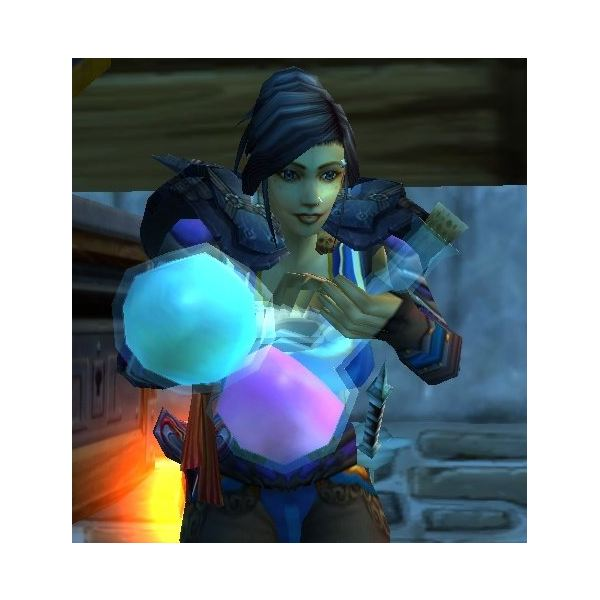
\includegraphics[width=0.4\textwidth]{figures/wow}
			\end{figure}
		\end{itemize}	
	\end{multicols}
\end{frame}	

\begin{frame}{Sparse K-Means Theory}
	Proposition: The solution to this convex problem is,
	\begin{align}\nonumber
		w_{jj} = \frac{(sign(a_{j})(|a_{j}|-\delta))_+}{(sign(a_{j})(|a_{j}|-\delta))^2_+}
	\end{align}	
	\noindent  where the $+$ subscript indicates the positive part of the function, $\delta = 0$ if that results in $\sum_{j=1}^{p} \abs{w_{jj}} < s$ or $\delta > 0$ is chosen so that $\sum_{j=1}^{p} \abs{w_{jj}} = s$ and it is assumed that $1 \leq s \leq \sqrt{p}$.
	\vspace{10mm}
	\begin{itemize}
		\centering
		\item<2-> \textbf{How do we find $\delta$?}
	\end{itemize}	
	\vspace{20mm}	
	\begin{tiny}
		\begin{noindlist}
			\item $[1]$ Witten, Daniela M., Robert Tibshirani, and Trevor Hastie. ``A penalized matrix decomposition, with applications to sparse principal components and canonical correlation analysis.'' Biostatistics 10.3 (2009): 515-534.
		\end{noindlist}
	\end{tiny}		
\end{frame}	

\begin{frame}{Sparse K-Means Theory}
	\begin{figure}[H]
		\centering
		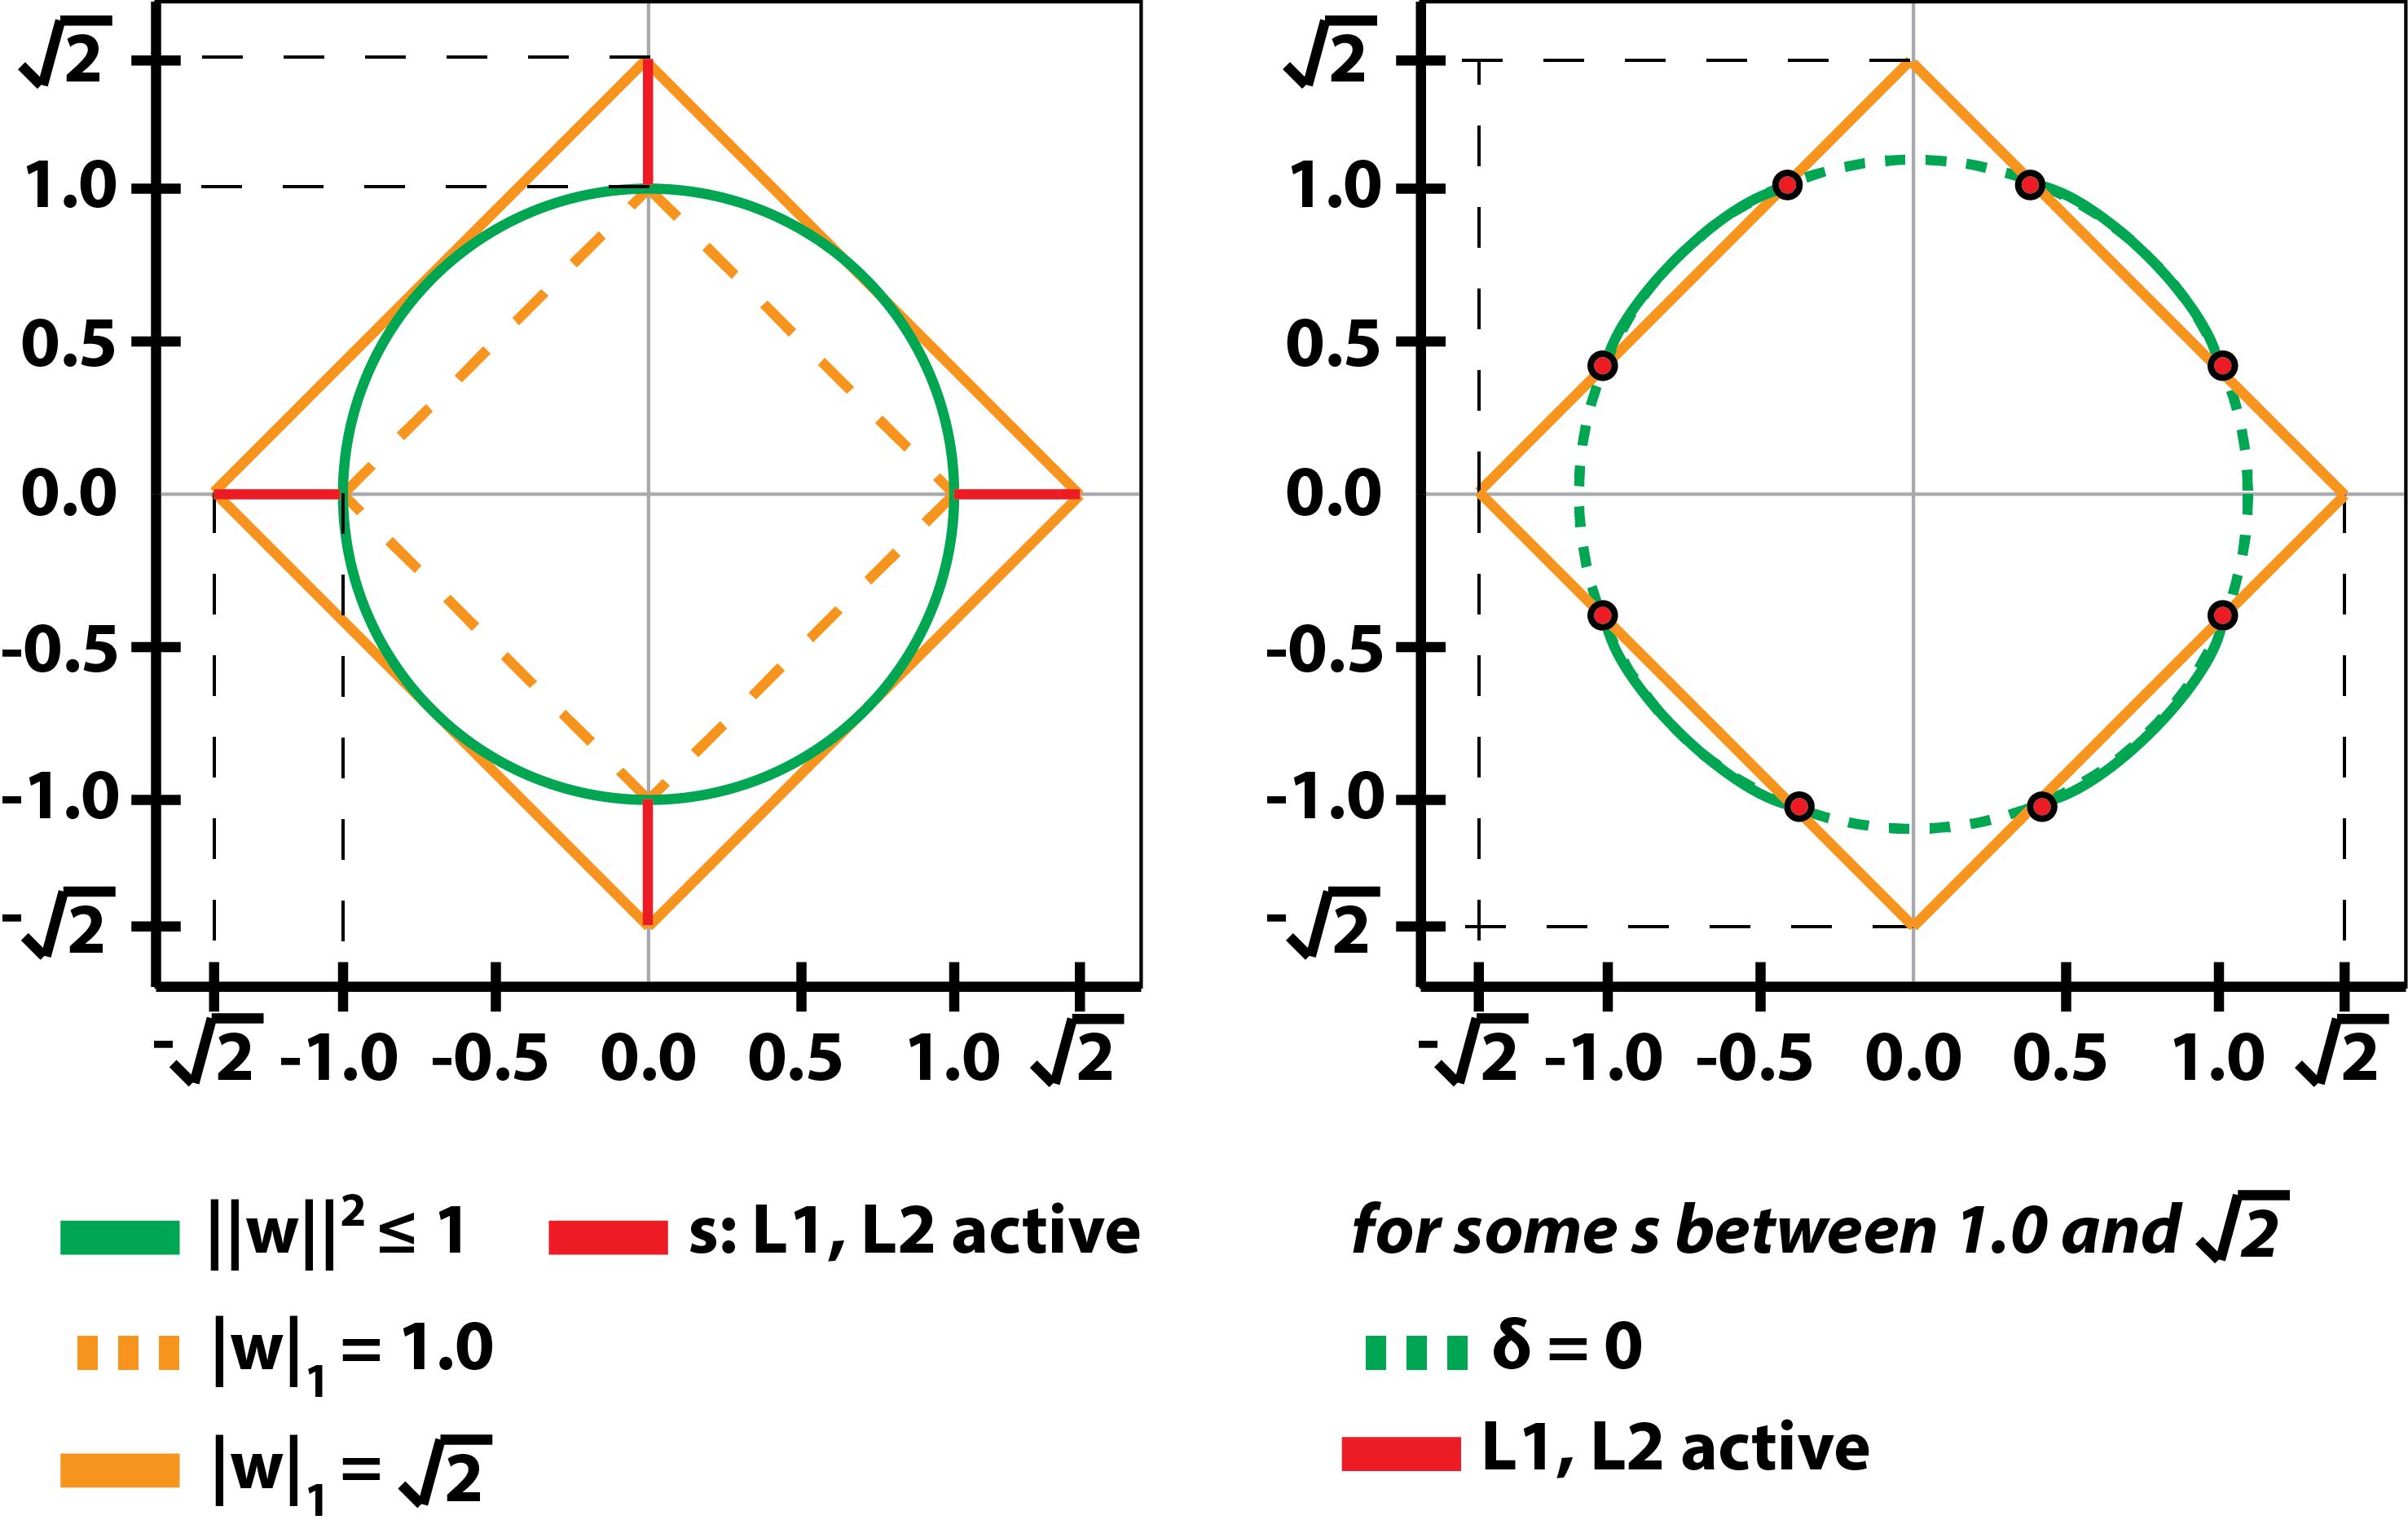
\includegraphics[width=0.9\textwidth]{figures/skm0}
	\end{figure}	
	\vspace{1mm}	
	\begin{tiny}
		\begin{noindlist}
			\item $[1]$ Witten, Daniela M., Robert Tibshirani, and Trevor Hastie. ``A penalized matrix decomposition, with applications to sparse principal components and canonical correlation analysis.'' Biostatistics 10.3 (2009): 515-534.
		\end{noindlist}
	\end{tiny}		
\end{frame}	

\begin{frame}{Sparse K-Means Theory}
	Using the Binary Search algorithm:
	\vspace{3mm}
	\begin{itemize}[label={\MyShadow{$\bullet$}{blue!80}}]
		\item Let $\delta$ be between $lim_1$ and $lim_2$
		\vspace{3mm}
		\item $lim_1 = 0$, $lim_2 = max(a)$
		\vspace{3mm}
		\item Iterate...
		\item[]
			\begin{align}\nonumber
				u = \frac{ \sum_{j=1}^p (sign(a_{j})(|a_{j}|-\frac{lim_1+lim_2}{2}))_+ } {\sum_{j=1}^p (sign(a_{j})(|a_{j}|-\frac{lim_1+lim_2}{2}))^2}
			\end{align}
			\begin{align}\nonumber
				\begin{Bmatrix}
					\lim_2 = \frac{lim_1+lim_2}{2} &, u < s \\ 
					\lim_1 = \frac{lim_1+lim_2}{2} &, u \geq s
				\end{Bmatrix}
			\end{align}
		\vspace{3mm}
		\item $\delta = \frac{lim_1+lim_2}{2}$
	\end{itemize}
\end{frame}	

\begin{frame}[plain,c]
	\begin{center}
		\Huge Sparse K-Means\\
		\Huge - Algorithm -
	\end{center}
\end{frame}

\begin{frame}{Sparse K-Means Algorithm}
	\textbf{Phase 1}\\
	\begin{figure}[H]
		\centering
		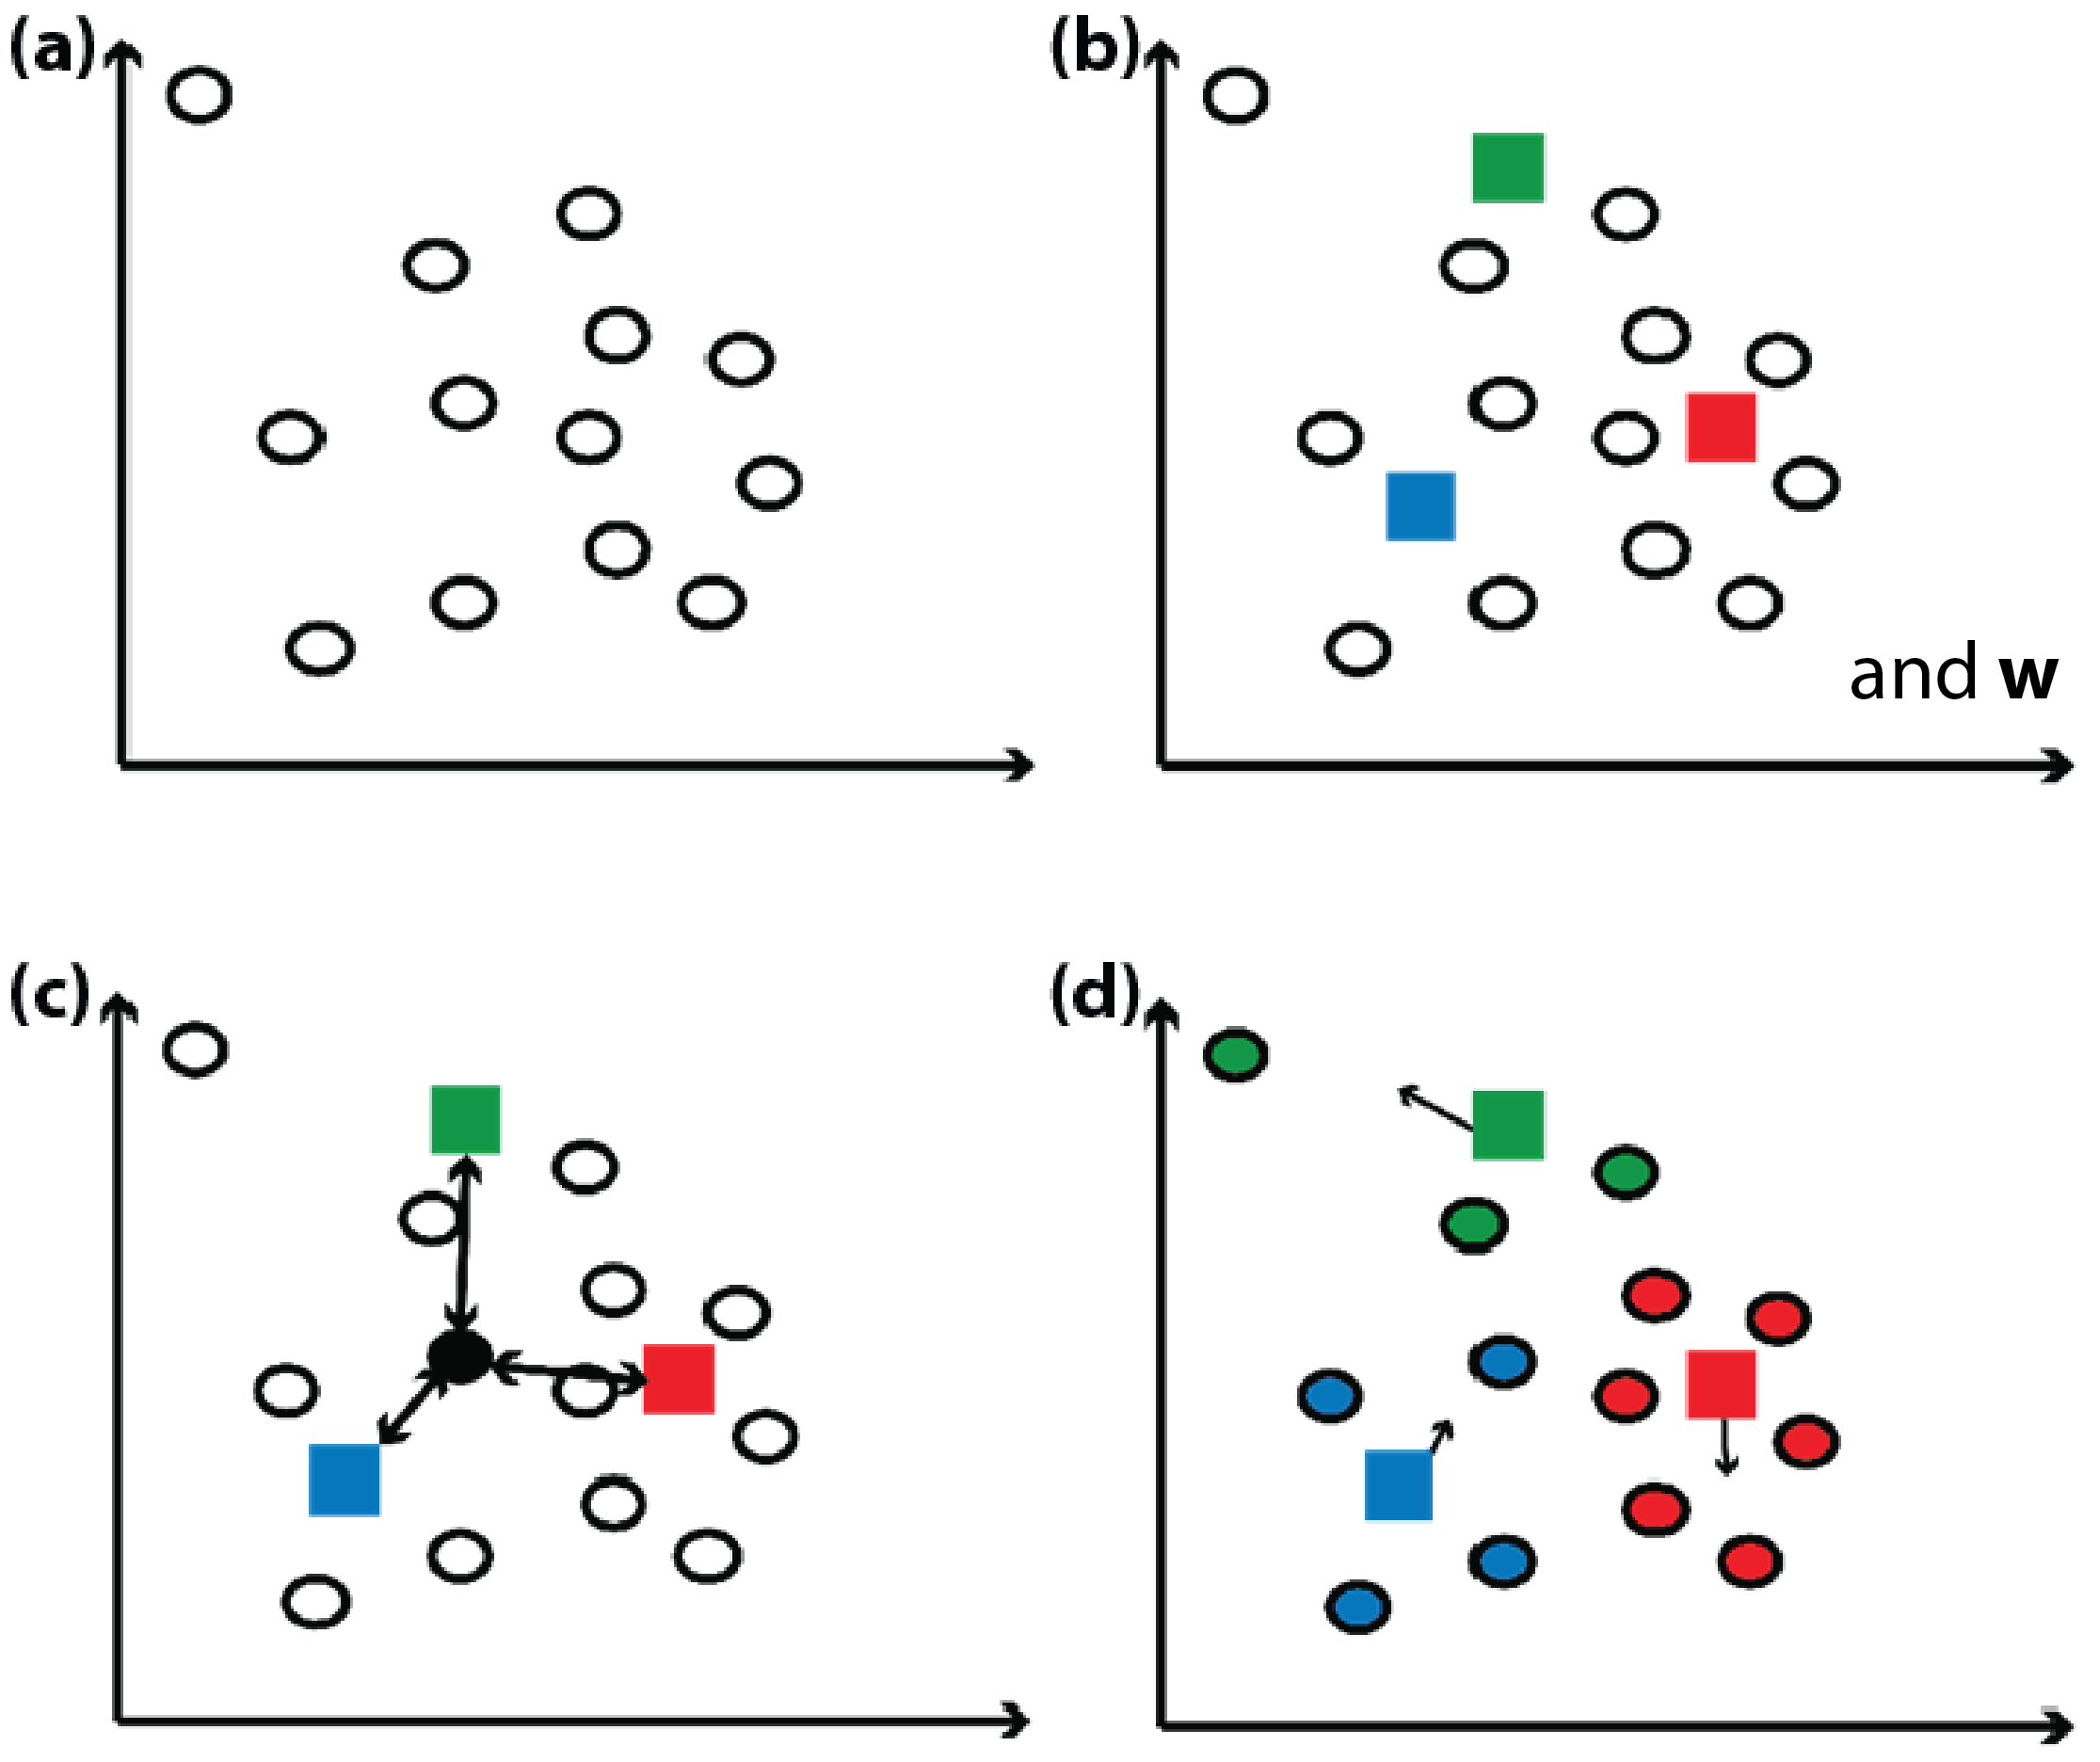
\includegraphics[width=0.7\textwidth]{figures/skm1}
	\end{figure}
\end{frame}

\begin{frame}{Sparse K-Means Algorithm}
	\textbf{Phase 2}\\
	\begin{itemize}[label={\MyShadow{$\bullet$}{blue!80}}]
		\item Execute Binary Search to find $\delta$\\i.e. $\delta = BinarySearch(wBCSS,s)$
		\vspace{3mm}
		\item Compute all the new weights using
			\begin{align}\nonumber
				w_{jj} = \frac{(sign(a_{j})(|a_{j}|-\delta))_+}{(sign(a_{j})(|a_{j}|-\delta))^2_+}
			\end{align}	
	\end{itemize}
	\textbf{Phase 3}\\
	\begin{itemize}[label={\MyShadow{$\bullet$}{blue!80}}]
		\item Update dataset based on $w$.
		\vspace{3mm}
		\item Repeat from \textbf{Phase 1c} until convergence.	
	\end{itemize}	
\end{frame}

\begin{frame}[plain,c]
	\begin{center}
		\Huge Sparse K-Means\\
		\Huge - Tuning -
	\end{center}
\end{frame}

\begin{frame}{Sparse K-Means Tuning}
	\textbf{How do we decide $k$ and $s$?}
	\vspace{3mm}
	\begin{itemize}[label={\MyShadow{$\bullet$}{blue!80}}]
		\item Normally for $k$ we use a performance index. But...
			\begin{multicols}{2}
				\begin{figure}[H]
					\centering
					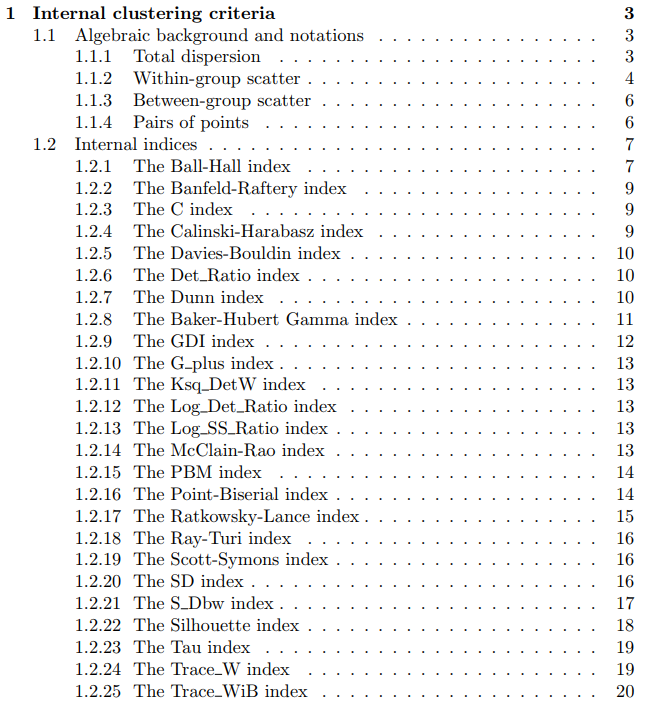
\includegraphics[width=0.45\textwidth]{figures/gap1}
				\end{figure}	
				\begin{tiny}
					\begin{noindlist}
						\item $[1]$ Desgraupes, Bernard. ``Clustering indices.'' University of Paris Ouest-Lab Modal’X 1 (2013): 34.	
					\end{noindlist}
				\end{tiny}	
				\vspace{2mm}
				\begin{itemize}[label={\MyShadow{$\bullet$}{blue!80}}]
					\item<2-> In the studies of [2] and [3] the gap statistic is proposed. But...
					\vspace{2mm}
					\begin{tiny}
						\begin{noindlist}
							\item $[2]$ Witten, Daniela M., and Robert Tibshirani. ``A framework for feature selection in clustering.'' Journal of the American Statistical Association 105.490 (2010): 713-726.
							\item $[3]$ Brodinova, Sarka, et al. ``Robust and sparse k-means clustering for high-dimensional data.'' arXiv preprint arXiv:1709.10012 (2017).		
						\end{noindlist}
					\end{tiny}
				\end{itemize}
			\end{multicols}
	\end{itemize}	
\end{frame}

\begin{frame}{The Gap Statistic}
	\begin{figure}[H]
		\centering
		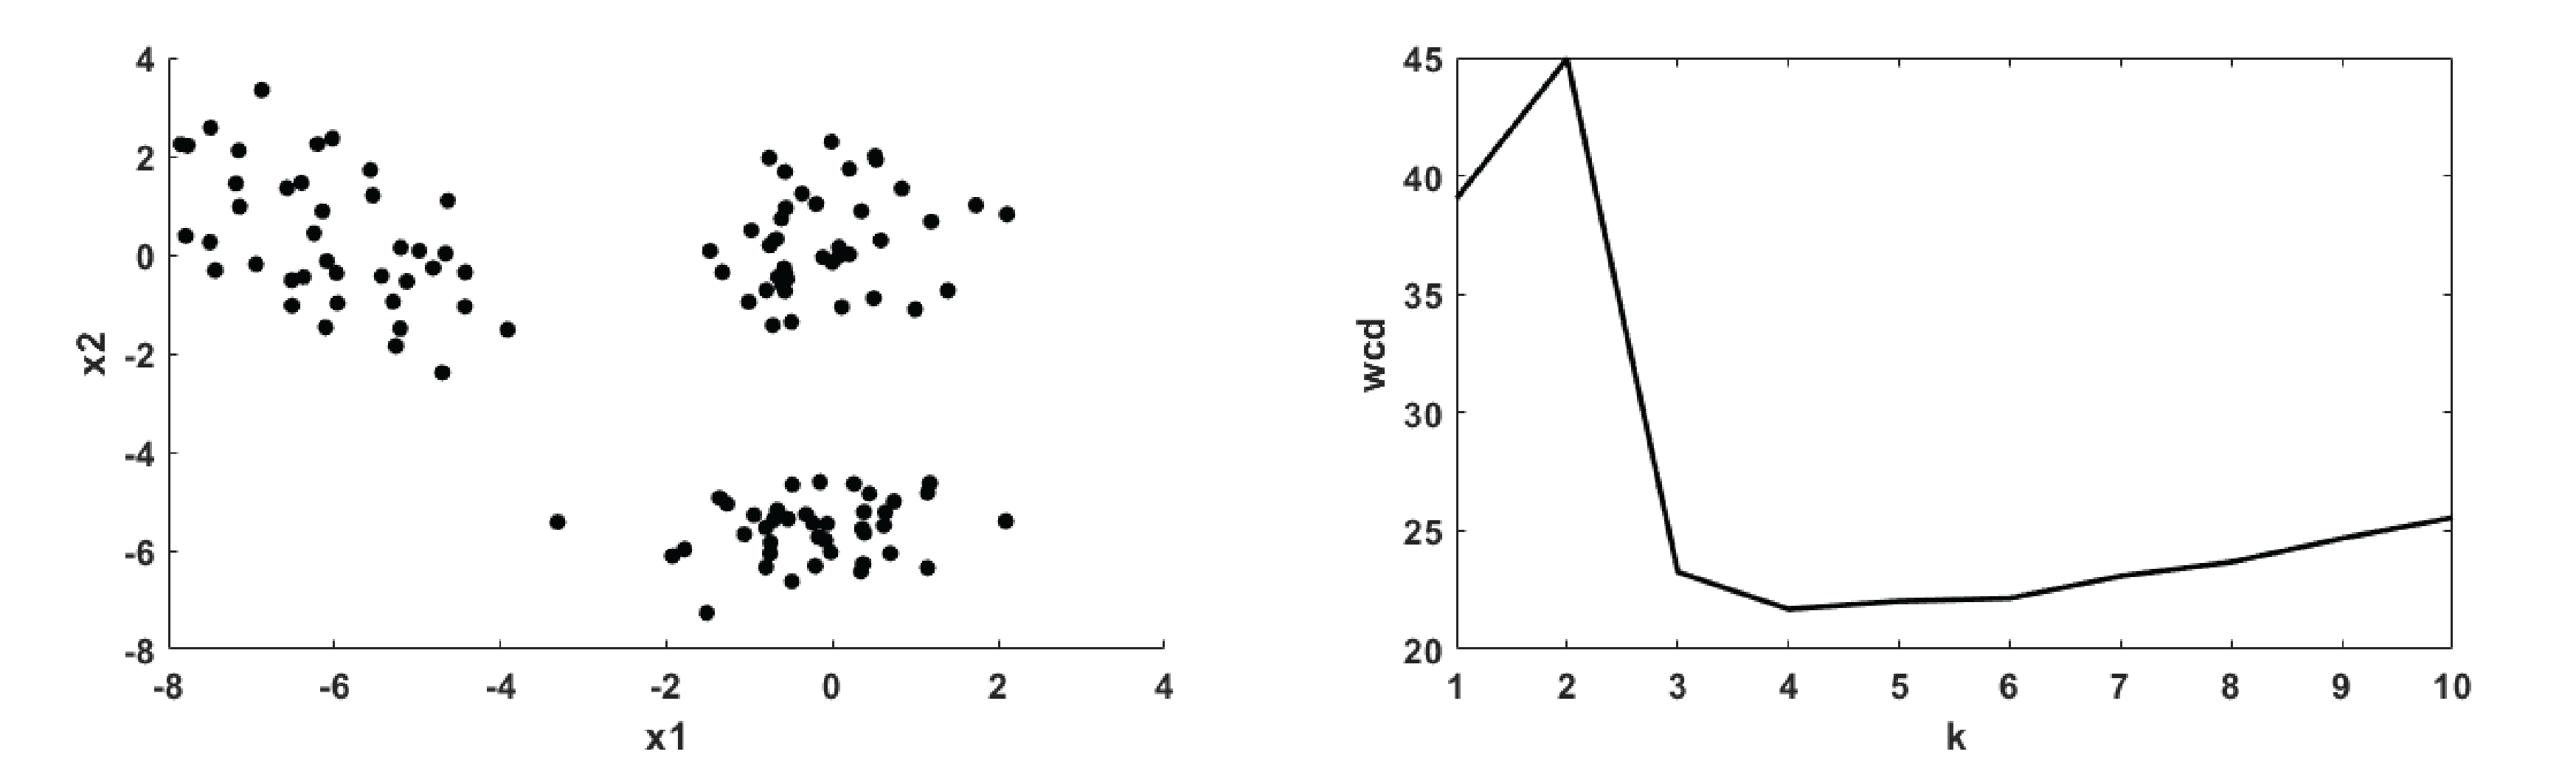
\includegraphics[width=\textwidth]{figures/gap2}
	\end{figure}
	\begin{tiny}
		\btVFill
		\begin{noindlist}
			\item $[1]$Tibshirani, Robert, Guenther Walther, and Trevor Hastie. ``Estimating the number of clusters in a data set via the gap statistic.'' Journal of the Royal Statistical Society: Series B (Statistical Methodology) 63.2 (2001): 411-423.
		\end{noindlist}
	\end{tiny}	
\end{frame}

\begin{frame}{The Gap Statistic}
	\begin{itemize}[label={\MyShadow{$\bullet$}{blue!80}}]
		\item Standardize the graph of $\log(WCSS_k)$ by comparing it with its expectation under an appropriate null reference distribution of the dataset.
		\vspace{3mm}
		\item The optimal number of clusters is then the $k$ for which $log(WCSS_k)$ falls the farthest below the reference curve.	
		\vspace{3mm}	
		\item $Gap_k = E_b^*\{\log(WCSS_k)\}-\log(WCSS_k)$
	\end{itemize}
	\begin{figure}[H]
		\centering
		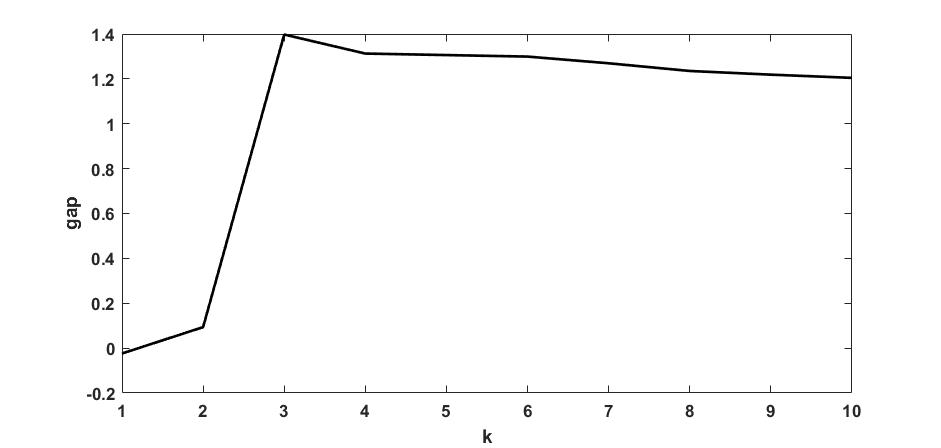
\includegraphics[width=0.75\textwidth]{figures/gap3}
	\end{figure}
\end{frame}

\begin{frame}{The Gap Statistic: Algorithm}
	\begin{itemize}[label={\MyShadow{$\bullet$}{blue!80}}]
		\item Given dataset $D$, cluster it with different values for $k$ and keep $\log(J_k)$, where $J_k$ specifies the final value of the objective function of the clustering algorithm for a given $k$.
		\item Create $B$ permutations of $D$ and for each repeat the above step, which results to: $\log(J_k^b) = [\log(J_k^1),\dots,\log(J_k^B)$, for each $k$.
		\item Compute the estimated gap statistic, 
		\begin{equation}\nonumber
		Gap_k = \frac{1}{B}\sum_{b=1}^{B}\log(J_k^b) - \log(J_k)
		\end{equation}
		\item Given that $E_b^* = \frac{1}{B}\sum_{b=1}^{B}\log(J_k^b)$, compute the simulation error,
		\begin{equation}\nonumber
		SE_k = \sqrt{\frac{1}{B}\sum_{b=1}^{B}\bigg(\log(J_k^b)-E_b^*\bigg)^2} + \sqrt{1+\frac{1}{B}}
		\end{equation}		
		\item Optimal $k$, $\hat{k}$, is the smallest $k$ for which $Gap_k \geq Gap_{k+1}-SE_{k+1}$ 
	\end{itemize}
\end{frame}

\begin{frame}{The Gap Statistic: Algorithm}
	\textbf{How many permutations, $B$?}
	\begin{itemize}[label={\MyShadow{$\bullet$}{blue!80}}]
		\item<2-> Witten, Daniela M., and Robert Tibshirani. ``A framework for feature selection in clustering.'' Journal of the American Statistical Association 105.490 (2010): 713-726. \textbf{B=25}.
		\vspace{3mm}	
		\item<2-> $[3]$ Brodinova, Sarka, et al. ``Robust and sparse k-means clustering for high-dimensional data.'' arXiv preprint arXiv:1709.10012 (2017). \textbf{B=10}.
		\item<3-> MATLAB, \textbf{B=100}.
		\vspace{3mm}	
		\item<3-> R, \textbf{B=100}.
	\end{itemize}
	\begin{itemize}[label={\MyShadow{$\bullet$}{red!80}}]
		\item<4-> Let's say $B = 45$. We would like to test 10 different values for $k$ and 5 for $s$.
		\item<5-> We need to execute our algorithmic framework, $45+1(B) \hphantom{x} x \hphantom{x} 10(k) \hphantom{x} x \hphantom{x} 5(s) = 2300$ times!
	\end{itemize}
\end{frame}

\begin{frame}[plain,c]
	\begin{center}
		\Huge Ongoing Research
	\end{center}
\end{frame}

\begin{frame}{Ongoing Research}
	\begin{figure}[H]
		\centering
		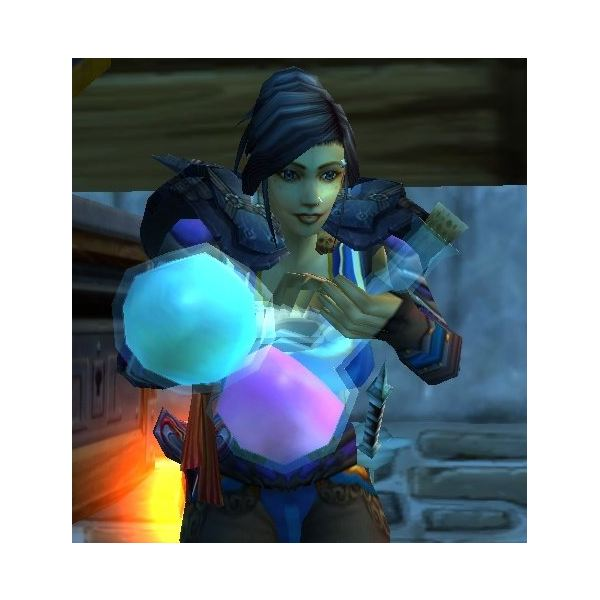
\includegraphics[width=0.4\textwidth]{figures/wow}
	\end{figure}
	\begin{itemize}[label={\MyShadow{$\bullet$}{blue!80}}]
		\item<2-> Find a computationally less expensive criterion than the gap statistic.
		\item<2-> Preliminarily results indicated that:
			\begin{itemize}[label={\MyShadow{$\star$}{blue!80}}]
				\item Silhouette index for $s$.
				\item Correlation for $k$.
			\end{itemize}
	\end{itemize}
\end{frame}



\end{document}

